\documentclass[a4paper]{article}

%--------------------------------------------------------------------------
\usepackage[a4paper, total={6in, 8in}]{geometry}
\usepackage{booktabs}
\usepackage{graphicx}
\usepackage{listings}
\usepackage{siunitx}

%--------------------------------------------------------------------------
\graphicspath{{./fig}}

%--------------------------------------------------------------------------
\begin{document}
\title{Udacity: Search and Sample Return Report}
\author{Shane Reynolds}
\maketitle
%--------------------------------------------------------------------------
\section{Introduction \& Background}
A simplistic and wide reaching definition of a robot is a machine which performs a task with some level of autonomy. In this context, robotic systems are appealing as they allow humans to avoid work that is considered dull, dirty and dangerous. This broad definition somewhat obfuscates the elements that make robotics work. Indeed, there is no clear consensus as to the mandatory sub-systems which comprise a robotic system, however, there are some common features which can be observed across many existing robotics platforms, these include:
\begin{itemize}
\item \textbf{Perception systems}: systems which allow the robot to perceive the world around it
\item \textbf{Decision making systems}: systems which allow the robot to decide a course of action given some information set
\item \textbf{Actuation systems}: systems which allow the robot to physically interact with the world
\end{itemize}

This project serves as a short introduction to these three systems. Principally, it touches on elementary image processing concepts, and very briefly explores some basic decision making. The project is based on a simulated mobile robot operating in a simple terrain environment. The simulation is built in Unity and main python script which gives the robot perception and decision making capabilities is called XXXX. Finally, the interface between image processing, decision making algorithms, and the simulation is driven by SocketIO. A screen shot of the simulation can be seen in Figure 1 below.

\begin{figure}
\centering
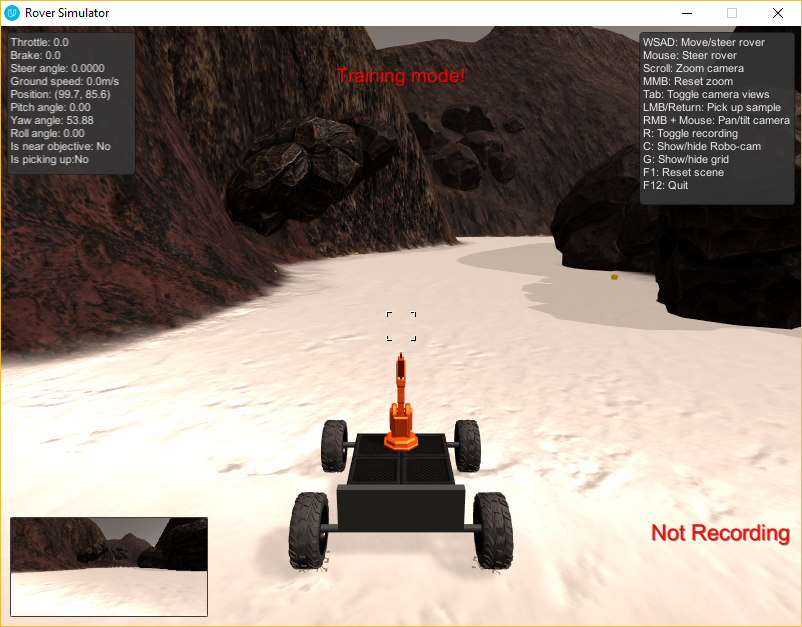
\includegraphics{image1}
\caption{A screenshot of the mobile robotic rover at a standstill in the simulated environment.}
\end{figure}

%--------------------------------------------------------------------------
\section{Methods and Implementation}
\subsection{Sensor Data}
The robot perceives its world via sensors. The main sensor used in this project is the camera mounted to the front of the robot. Figure 2 shows an example of a single image captured from the rover's camera. The camera images are received approximately once every 27$\si{\milli\second}$, or 36$\si{\hertz}$.

\begin{figure}
\centering
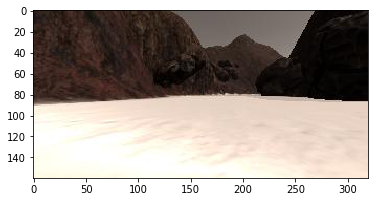
\includegraphics{image2}
\caption{A single image of the simulated environment as shown from the robot's front mounted camera.}
\end{figure}

In addition to the camera data, the there are sensors which measure the rover's position and orientation in space. Position is given by simple Cartesian coordinates, $(x, y)$, with reference to a fixed world frame. Orientation is given by roll, pitch, and yaw which are also with reference to the fixed world frame. Finally, throttle, brake, and steering angle of the rover are also provided. These values values are received at the same frequency as the images. The sensor data is used to help determine a course of action for the robot. This is achieved with two principal functions: \verb|perception_step| and \verb|decision_step|. Table 1 shows the different sensors data types, and a basic description of use of the captured data. 

\begin{table}
\caption{A table which shows the different sensor data types, and their python format.}
\begin{tabular}{llp{10cm}}
\toprule
\textbf{Sensor Data Type} & \textbf{Python Variable} & \textbf{Description}\\
\midrule
Image & \verb|img| & The image which is captured by the rover's front mounted camera - it is an \verb|np.array| of dimension $(160,320,3)$ and type \verb|uint8|\\
Position & \verb|pos| & Position of the rover with respect to a fixed world coordinate frame - it is a tuple of type \verb|np.float| \\
Yaw & \verb|yaw| & 	The yaw of the rover with respect to the world coordinate frame - it is of type \verb|np.float| and is one part of the rover orientation description\\
Pitch & \verb|pitch| & The pitch of the rover with respect to the world coordinate frame - it is of type \verb|np.float| and is one part of the rover orientation description\\
Roll & \verb|roll| & The roll of the rover with respect to the world coordinate frame - it is of type \verb|np.float| and is one part of the rover orientation description\\
Current Velocity & \verb|velocity| & The velocity of the rover - is of type \verb|np.float| and is capped at 2$\si{\meter\per\second}$ in this project\\
Steering Angle & \verb|steer| & The steering angle of the rover is determined by the angle of the front wheels with the centre line axis of the rover - is of type \verb|np.float| and is bound between $\pm 15 \si{\deg}$\\
Throttle Value & \verb|throttle| & Represents the value of locomotive force applied by the rover motors - is of type \verb|np.float| and is binary in opearation in that throttle is either applied, or not\\
Brake Value & \verb|brake| & Represents the applied force opposing motion (due to friction)
\bottomrule
\end{tabular}
\end{table}

%--------------------------------------------------------------------------
\subsection{Image Processing}
Image processing represents a large component of the project, and consists of multiple stages. It is encapsulated in the \verb|perception_step| function, and is applied to each image captured by the rover's front mounted camera. The processing consists of three principal components: perspective transformation, segmentation, and translating the image to obtain a rover centric coordinate system. There is no fixed order in which the perspective transformation and segmentation steps need to occur, however, the transformation to a rover centric coordinate system can only be performed once the image has undergone a perspective transformation. The following subsections decribe each component in more detail.

%--------------------------------------------------------------------------
\subsubsection{Perspective Transformation}
To make navigation easier to comprehend for observers of the rover behaviour, it is often useful to implement a perspective transforms. Certainly, the rover is capable of navigating via the front mounted RGB camera, however, it is often useful to transform this view into a top down perspective. The process for implementing such a transform involves the following four steps:
\begin{enumerate}
\item Define four $(x,y)$ points in the source image (the image from the front mounted camera);
\item Identify the four $(x,y)$ points, defined from the source image, in the destination image (the top down image);
\item Using the information from steps 1) and 2), create a transformation matrix which will transform the points from the source image to the destination image;
\item Apply the transformation matrix to captured image arrays to convert the images from the front mounted camera to a top down perspective.
\end{enumerate}  

The Often is it useful to apply a grid of known size to both the source and destination images to help with the identification of points in each image. The grid applied in this instance was a 1$\si{\meter}$ by 1$\si{\meter}$ grid, and can be seen in Figure 3. The points used in both the source image and destination image to build the transformation matrix can be seen in Table 2, and the code snippet showing the creation of the transformation matrix can be seen in Figure 4. Finally, once the transformation matrix is determined, then it can be applied to each received image to transform the perspective from the front mounted camera to the top down view - a demonstration of this can be seen in Figure 5. It is worth noting that it should be expected that the perspective transform will have regions of black present in transformed image - these black areas represent the rover's blind spots.

\begin{figure}
	\begin{minipage}{0.45\linewidth}
		\begin{table}
		\caption{The points determined from the destination and source images use to create the perspective transformation matrix.}
		\begin{tabular}{ll}
		\toprule
		\textbf{Source} & \textbf{Destination}\\
		\midrule
		P1 & P1\\
		P1 & P1\\
		P1 & P1\\
		P1 & P1\\
		\bottomrule
		\end{tabular}
		\end{table}
	\end{minipage}
	\begin{minipage}{0.45\linewidth}
		\begin{lstlisting}[language=Python]

		\end{lstlisting}
		\caption{Code snippet of the perspective transform}
	\end{minipage}
\end{figure}

\begin{figure}
	\centering
	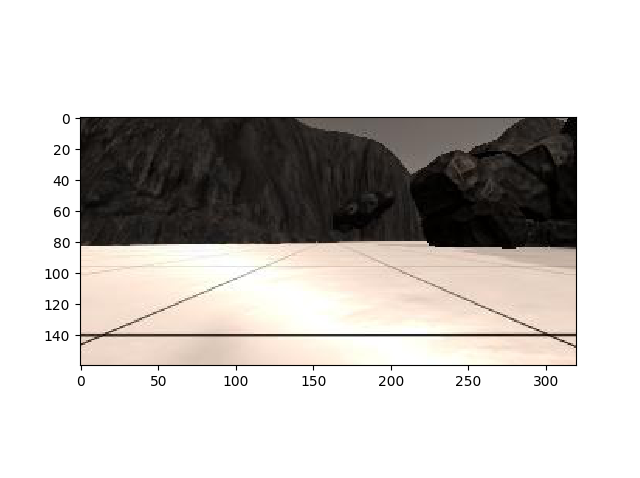
\includegraphics[scale=0.5]{image3}
	\caption{text}
\end{figure}

\begin{figure}
	\centering
	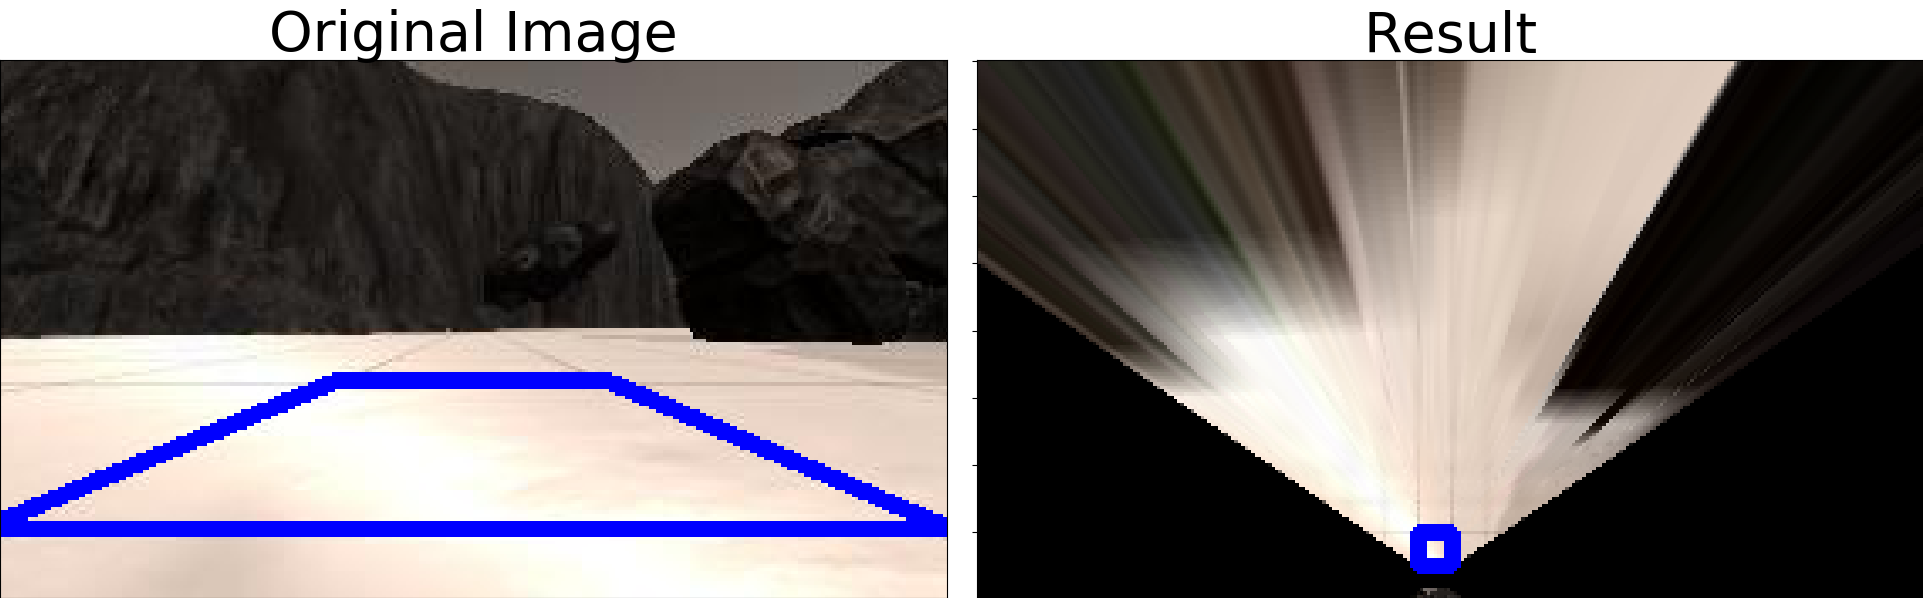
\includegraphics[scale=0.5]{image4}
	\caption{text}
\end{figure}

\subsubsection{Segmentation: Navigable Terrain \& Obstacles}
There are 3 different types of object that are of interest to the rover: navigable terrain, obstacles, and rock samples. A simple way to obtain the navigable terrain is to create a basic RGB filter. This works because it exploits the stark contrast between obstacles (which are dark), and navigable terrain (which is light). We are able to extract both navigable terrain and obstacles with one instance of filtering since these two types of terrain are mutually exclusive - to put this simply: if the terrain is not navigable, then it must be an obstacle. The filtering itself is simplistic in its implementation, using an upper threshold for each of the R, G, and B values. To determine the cut-off threshold for each of the R, G, and B channels, most Operating Systems come with a basic image viewer which will provide information for each of the R, G, and B channels by pixel. A single frame of navigable terrain was loaded into an image viewer. Using this crude analysis values of 160 for each of the R, G, and B channels were determined as an appropriate threshold for navigable terrain. This process is shown in Figure 5. If a pixel in an image has R, G, and B values which are all greater than 160, the pixel is classified as navigable terrain. If this criterion is not satisfied, then the pixel is classified as an obstacle. The implementation of this code can be seen below.

\begin{lstlisting}[language=Python]

\end{lstlisting}

\begin{figure}
\begin{minipage}{0.45\linewidth}
\centering
\caption{Include a grpahic of the original image}
\end{minipage}
\begin{minipage}{0.45\linewidth}
\centering
\caption{Include a graphic of the terrain being filtered - gray scale}
\end{minipage}
\end{figure}

This section is more curious that that. If we filter prior to transforming, then there is some distortion to the filtered image. Basically determined what the cone is and subtracted this from the transformation to ge the final image. Further, some spacing has been left in between the navigable terrain and the obstacles to provide for a margin of error.

\begin{figure}
\centering
\caption{include a graphic of the final terrain being filtered for obstacles and }
\end{figure}

PERHAPS TEST: see what happens if the segmentation is made first and then the transformation is made leaving an image gap - if there is no distortion then this may be the better solution.

\subsubsection{Segmentaiton: Rock Samples}
To get the rock samples it was a little harder - the RBG did not work that well and instead HSV was used. Talk some about the RGB background and then talk some about the HSV background. Once the rocks have been determined they are added to the image

CODE SNIPPET

\begin{figure}
\begin{minipage}{0.45\linewidth}
\centering
\caption{include a graphic of the original rock image}
\end{minipage}
\begin{minipage}{0.45\linewidth}
\centering
\caption{include a graphic of the filtered image - gray scale}
\end{minipage}
\end{figure}

\begin{figure}
\centering
\caption{Include an image of the full image transformation with the rock and the blue and green}
\end{figure}

\subsubsection{Rover Centric Coordinates}
Transformation of the image into a rover centric coordinate frame. The transformed image needs to be attached to the rover centric coordinate frame - this needs more explaining exactly what is happening here with the transformed image. What is it doing and why do we do it?

CODE SNIPPET

\begin{figure}
\begin{minipage}{0.45\linewidth}
\centering
\caption{include a non-transformed image}
\end{minipage}
\begin{minipage}{0.45\linewidth}
\centering
\caption{include an image of the transformed rover centric coord system}
\end{minipage}
\end{figure}

\subsubsection{Writing Colour Map to the World Map}

Updates the map. Describe what is actually happening here? This has not yet been described - essentially what we have is an image and we want to update the ground truth of the world map as the rover explores autonomously.

CODE SNIPPET

\begin{figure}
\centering
\caption{Show a picture of the mapped terrain, if possible}
\end{figure}

%--------------------------------------------------------------------------
\subsection{Autonomous Navigation}
\subsubsection{Perception Step}
Need to talk about the implementation of these sections of the code

\subsubsection{Decision Step}
Need to talk about the implementation of these sections of the code

%--------------------------------------------------------------------------
\section{Results \& Conclusion}

%--------------------------------------------------------------------------
\section{Further Enhancements}

\end{document}